\documentclass{beamer}

\usetheme{Padova}
\usepackage[absolute,overlay]{textpos}
\usepackage{float}
\usepackage[utf8]{inputenc}

\subtitle{Dipartimento di Matematica "Tullio Levi-Civita"\\
Corso di Laurea in Informatica}
\title{Implementazione di una interfaccia SAPI 5 mediante i sistemi di sintesi vocale MaryTTS e Speect }
\author{Laureando: Cristian Andrighetto\\
		Relatore: Paolo Baldan}
\date{20 Luglio 2017}


\begin{document}

	\maketitle

	\section{L'azienda}

	\begin{frame}{L'azienda}

		\begin{figure}[H]
			\centering
			
\includegraphics{images/logo-mivoq.png}
		\end{figure}
	
		\begin{itemize}
			\item sede a Padova all'interno dell'Istituto di Scienze e Tecnologie della Cognizione (ISTC) che fa parte del CNR
			\item tecnologie vocali
			\item personalizzazione della voce
			
		\end{itemize}
	\end{frame}

	\section{Sintesi Vocale}
	
	\begin{frame}{Sintesi Vocale}
		\begin{textblock*}{5cm}(1cm,2cm) % {block width} (coords)
			
\includegraphics[width=5cm]{images/marylogo}
		\end{textblock*}
		\begin{textblock*}{5cm}(7cm,2cm) % {block width} (coords)
			
\includegraphics[width=5cm]{images/speect_logo_full}
		\end{textblock*}
		\begin{itemize}
			\item piattaforma \textbf{FATTS} che integra \textbf{MaryTTS} (prodotto attuale)
			\item sviluppo dell'engine TTS \textbf{Speect} (prossimo prodotto)
		\end{itemize}
	\end{frame}


	\section{Problema affrontato}

	\begin{frame}{Problema affrontato}
		Integrazione degli \textbf{engine Text-To-Speech} con \textbf{Microsoft Windows} attraverso interfaccia \textbf{SAPI 5}
		\begin{itemize}
		\item \textbf{rendere funzionanti} gli engine TTS con Microsoft Windows
		\item \textbf{studiare} l'interfaccia SAPI 5 per trovare la soluzione migliore
		\end{itemize}
		\vspace{10pt}
		Aggiungere funzionalità a \textbf{Speect}
		\begin{itemize}
			\item regolazione \textbf{tonalità} voce
			\item regolazione \textbf{velocità} voce
		\end{itemize}
	\end{frame}

	\section{Soluzione}
	
	\begin{frame}{Soluzione}
		Per \textbf{MaryTTS}
		\begin{itemize}
			\item implementazione di una interfaccia SAPI 5
			\item componente per la comunicazione con MaryTTS
		\end{itemize}
		Per \textbf{Speect}
		\begin{itemize}
			\item implementazione di una interfaccia SAPI 5
		\end{itemize}
	\end{frame}

	\section{Architettura per MaryTTS}
	
	\begin{frame}{Architettura per MaryTTS}
		\begin{figure}[H]
			\centering
			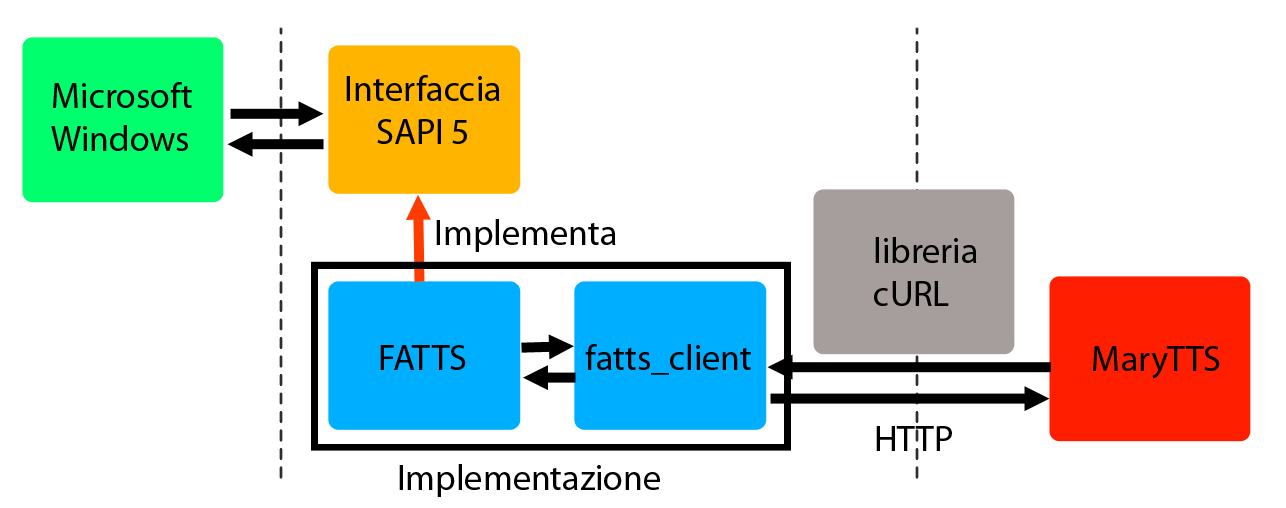
\includegraphics[width=\textwidth]{images/FATTS-sapi5.png}
		\end{figure}
	\end{frame}

	\section{Architettura per Speect}
	
	\begin{frame}{Archittetura per Speect}
		\begin{figure}[H]
			\centering
			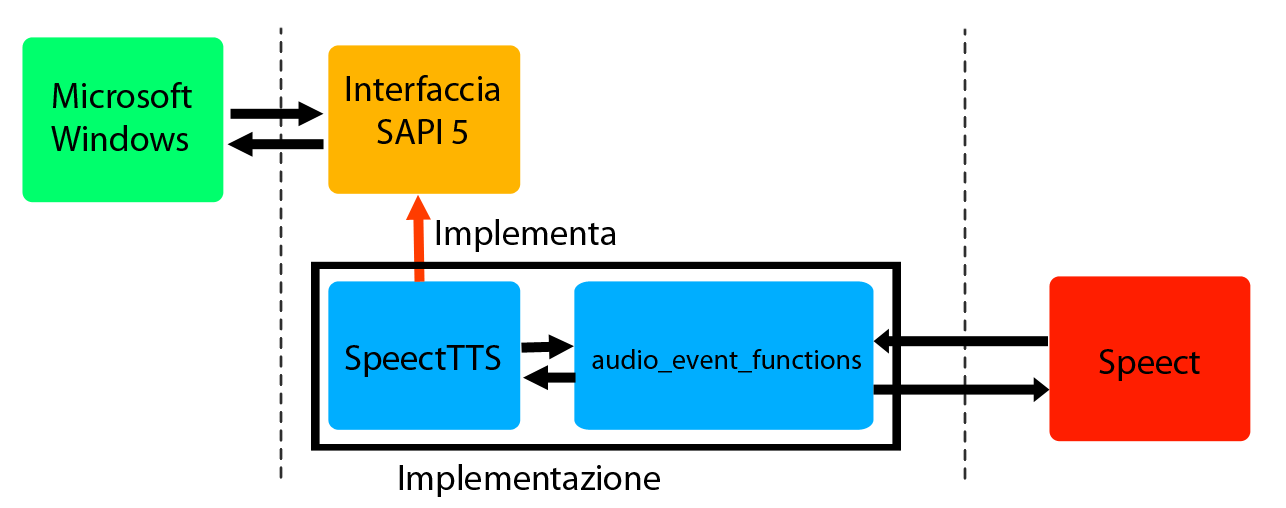
\includegraphics[width=\textwidth]{images/SpeectTTS-sapi5.png}
		\end{figure}
	\end{frame}
	

	


\end{document}
